\documentclass{article}

\usepackage[utf8]{inputenc}
\usepackage{amsmath}
\usepackage{amsfonts}
\usepackage{amssymb}
\usepackage{tikz}
\usepackage{tkz-euclide}


\newtheorem{theorem}{Theorem}

\author{Abegà Razafindratelo}
\title{Notes on Galileo Galilei Theorems}

\begin{document}

\maketitle

\section*{Abstract}

The purpose of this article is to explore some of \textit{Galileo Galilei} theorems in his famous book on dynamic mechanics \textit{Dialogues Concerning Two New Sciences}\cite{galilei_two_new_sciences} and do their demonstrations in a modern way.



\section*{Introduction}
In his book \textit{The two New Sciences}
\section{On the Salviati lemma}
\qquad On the \textit{Third day, Change of position, [De Motu Locali]}, Galileo explores the fundamental principles of motion and acceleration, laying the foundations of \textit{dynamical mechanics}.\\

\quad	One of the most significant theorems he presents in this \textit{Third day} is stated by \textit{Salviati} immediately after the \textit{Scholium} of the \textit{Corollary II} on page 183-184\\

\begin{theorem}
If a body falls freely along smooth planes inclined at any angle whatsoever, but of the same height, the speeds with which it reaches the bottomare the same.
\end{theorem}

\quad Galileo’s demonstration of this theorem follows an old mathematical approach, with expressions and notations that may be difficult to grasp. In the following, I will reformulate and prove the theorem using modern notation and clearer expressions, making the demonstration more accessible and easier to understand.\\

\begin{proof}
Let \textit{ABC} be a rectangle triangle.\\

Let $(AB)$ and $(AE)$ be inclined plane where the body may fall from the vertex $A$ to $B$ or $E$ according to the inclination of the plane.\\

In what follows, let $\alpha$ be the angle of inclination of the plane $(AB)$ and $\beta$ that of $(AE)$. Let $v_1$ represents the speed of the body falling from $A$ to $B$ according to time $t_1$ and $v_2$ the speed of the body falling from $A$ to $E$ according to time $t_2$.

\begin{figure}[h!]
    \centering
    $$
	\begin{tikzpicture}

    \tkzDefPoints{0/0/C, 4/0/B, 0/3/A}
    \tkzDefMidPoint(B,C) 
    \tkzGetPoint{E}

    \tkzDrawPolygon(A,B,C)

    \tkzDrawSegment(A,E)

    \tkzLabelPoints[below](C,B,E)
    \tkzLabelPoints[left](A)

    \tkzMarkRightAngle(A,C,B)

    \tkzMarkAngle[size=0.6](A,B,C)
    \tkzLabelAngle[pos=1.2](A,B,C){$\alpha$}

    \tkzMarkAngle[size=0.6](A,E,C)
    \tkzLabelAngle[pos=1.2](A,E,C){$\beta$}

	\end{tikzpicture}    
    $$
    \caption{Inclined plane}
    \label{fig:triangle_ABC}
\end{figure}


Let us lay down :
\[
\begin{cases}
AC = h	\\
AB = x_1\\
AE = x_2;	
\end{cases}
\] 

As we know :
\[
\begin{cases}

\sin{\alpha} = \frac{h}{x_1} \\
\sin{\beta} = \frac{h}{x_2}

\end{cases}
\]


That gives us :
\[
\begin{cases}
h = x_1\sin{\alpha}\\
h = x_2\sin{\beta}
\end{cases}
\]
As we know $  x_1 = \frac{1}{2}\cdot a_1\cdot t_1^{2}	$ where $ a_1 $ is the acceleration on the plane $ AB $, and $ t_1 $ the time required to travers it; and $ x_2 = \frac{1}{2}\cdot a_2\cdot t_2^{2} $. where $ a_2 $ the acceleration on the plane $ AE $, and $ t_2 $ the time required to travers that plane. \\

Now :
\begin{figure}[h!]
    \centering
	$$
	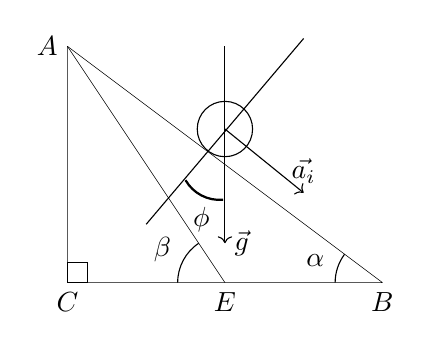
\begin{tikzpicture}

    \tkzDefPoints{0/0/C, 4/0/B, 0/3/A, 2/1.95/O}
    \tkzDefMidPoint(B,C) 
    \tkzGetPoint{E}

    
    \tkzDrawPolygon(A,B,C)

    \tkzDrawSegment(A,E)

    \tkzLabelPoints[below](C,B,E)
    \tkzLabelPoints[left](A)

    \tkzMarkRightAngle(A,C,B)
    

	\draw[->] (2,1.95) -- (3,1.14) node[below, above] {$\vec{a_i}$};
	\draw[->] (2,1.95) -- (2,0.5) node[below, right] {$\vec{g}$};
	\draw	(1,0.74)	--	(3, 3.1);

	
	\draw	(2,3)	--	(2,0.6);
	
	\draw[thick] (1.5, 1.3) arc[start angle=-150,end angle=-85,radius=0.5];
	\node at (1.7,0.8) {$\phi$};
	
    \tkzMarkAngle[size=0.6](A,B,C)
    \tkzLabelAngle[pos=0.9](A,B,C){$\alpha$}
    \tkzMarkAngle[size=0.6](A,E,C)
    \tkzLabelAngle[pos=0.9](A,E,C){$\beta$}


    \node[draw, circle, minimum size=20pt] at (2, 1.95) {};

	\end{tikzpicture}
	$$
    \caption{Falling body on the inclined plane}
    \label{fig:triangle_ABC}
\end{figure}
\newline
So, as we have : $a_i = g \sin{\phi}$, we have :
\[
\begin{cases}
x_1 = \frac{1}{2} a_1 t_1^{2}

=\frac{1}{2}  g t_1^{2} \sin{\alpha} \\

x_2 = \frac{1}{2}  a_2 t_2^{2}

=\frac{1}{2} g t_2^{2} \sin{\beta} \\
\end{cases}
\]

\[
\Longrightarrow
\begin{cases}
h = \left(
\frac{1}{2} g t_1^{2} \sin{\alpha}
\right)\cdot \sin{\alpha}

= \frac{1}{2} gt_1^{2} \sin^{2}{\alpha}	\\

h = \left(
\frac{1}{2} g t_2^{2} \sin{\beta}
\right)\cdot \sin{\beta}

= \frac{1}{2}  g t_2^{2} \sin^{2}{\beta}	\\
\end{cases}
\]

\[
`\Longrightarrow \quad
\frac{1}{2} g t_1^{2} \sin^{2}{\alpha} = \frac{1}{2}  g t_2^{2} \sin^{2}{\beta}	\\
\]
\[
\Longleftrightarrow \quad	 t_1^{2} \sin^{2}{\alpha} = t_2^{2} \sin^{2}{\beta} \\
\]
\[
\Longleftrightarrow \quad	t_1 \sin{\alpha} = t_2 \sin{\beta}	\\
\]
because time and distance (since $t$ and $h$ are both positive)
\begin{equation}
\Longleftrightarrow \quad	\frac{t_1}{t_2} = \frac{\sin{\beta}}{\sin{\alpha}}
\end{equation}

Now, in the other hand, the speeds of the body at the bottoms of each inclined plane is given by :
\[
\begin{cases}
v_1 = a_1t_1 \\
v_2 = a_2t_2 
\end{cases} \\
\Longrightarrow	\qquad
\begin{cases}
v_1 = g  t_1 \sin{\alpha} \\
v_2 = g  t_2 \sin{\beta}
\end{cases}
\]
Now, seing that each term of those equation are not null, by dividing term by term we have :
\[
\Longrightarrow	\qquad
\frac{v_1}{v_2} = \frac{g t_1 \sin{\alpha} }{g t_2 \sin{\beta}} = \frac{t_1 \sin{\alpha}}{t_2 \sin{\beta}}
\]

According to equation (1) we get :
\[
\frac{v_1}{v_2} = \frac{\sin{\alpha} }{\sin{\beta}} \times \frac{\sin{\beta} }{\sin{\alpha}} = 1
\]

\begin{equation}
\text{Therefore,} \qquad v_1 = v_2
\end{equation}

\end{proof}




\bibliographystyle{plain}
\bibliography{ref}

\end{document}